\documentclass{beamer}
\usepackage{amsmath}
\usepackage[english]{babel} %set language; note: after changing this, you need to delete all auxiliary files to recompile
\usepackage[utf8]{inputenc} %define file encoding; latin1 is the other often used option
\usepackage{csquotes} % provides context sensitive quotation facilities
\usepackage{graphicx} %allows for inserting figures
\usepackage{booktabs} % for table formatting without vertical lines
\usepackage{textcomp} % allow for example using the Euro sign with \texteuro
\usepackage{stackengine}
\usepackage{wasysym}
\usepackage{tikzsymbols}
\usepackage{textcomp}
% ELIMINAR COMANDOS DE NAVEGACION%%%%%%%%%%%
\setbeamertemplate{navigation symbols}

%\newcommand{\bubblethis}[2]{
 %       \tikz[remember picture,baseline]{\node[anchor=base,inner sep=0,outer sep=0]%
 %       (#1) {\underline{#1}};\node[overlay,cloud callout,callout relative pointer={(0.2cm,-0.7cm)},%
 %       aspect=2.5,fill=yellow!90] at ($(#1.north)+(-0.5cm,1.6cm)$) {#2};}%
 %   }%
%\tikzset{face/.style={shape=circle,minimum size=4ex,shading=radial,outer sep=0pt,
 %       inner color=white!50!yellow,outer color= yellow!70!orange}}

%% Some commands to make the code easier
\newcommand{\emoticon}[1][]{%
  \node[face,#1] (emoticon) {};
  %% The eyes are fixed.
  \draw[fill=white] (-1ex,0ex) ..controls (-0.5ex,0.2ex)and(0.5ex,0.2ex)..
        (1ex,0.0ex) ..controls ( 1.5ex,1.5ex)and( 0.2ex,1.7ex)..
        (0ex,0.4ex) ..controls (-0.2ex,1.7ex)and(-1.5ex,1.5ex)..
        (-1ex,0ex)--cycle;}
\newcommand{\pupils}{
  %% standard pupils
  \fill[shift={(0.5ex,0.5ex)},rotate=80] 
       (0,0) ellipse (0.3ex and 0.15ex);
  \fill[shift={(-0.5ex,0.5ex)},rotate=100] 
       (0,0) ellipse (0.3ex and 0.15ex);}

\newcommand{\emoticonname}[1]{
  \node[below=1ex of emoticon,font=\footnotesize,
        minimum width=4cm]{#1};}
\usepackage{scalerel}
\usetikzlibrary{positioning}
\usepackage{xcolor,amssymb}
\newcommand\dangersignb[1][2ex]{%
  \scaleto{\stackengine{0.3pt}{\scalebox{1.1}[.9]{%
  \color{red}$\blacktriangle$}}{\tiny\bfseries !}{O}{c}{F}{F}{L}}{#1}%
}
\newcommand\dangersignw[1][2ex]{%
  \scaleto{\stackengine{0.3pt}{\scalebox{1.1}[.9]{%
  \color{red}$\blacktriangle$}}{\color{white}\tiny\bfseries !}{O}{c}{F}{F}{L}}{#1}%
}
\usepackage{fontawesome} % Social Icons
\usepackage{epstopdf} % allow embedding eps-figures
\usepackage{tikz} % allows drawing figures
\usepackage{amsmath,amssymb,amsthm} %advanced math facilities
\usepackage{lmodern} %uses font that support italic and bold at the same time
\usepackage{hyperref}
\usepackage{tikz}
\usepackage{tcolorbox}

\usefonttheme[onlymath]{serif} %set math font to serif ones

\definecolor{beamerblue}{rgb}{0.2,0.2,0.7} %define beamerblue color for later use

%%% defines highlight command to set text blue
\newcommand{\highlight}[1]{{\color{blue}{#1}}}


%%%%%%% commands defining backup slides so that frame numbering is correct

\newcommand{\backupbegin}{
   \newcounter{framenumberappendix}
   \setcounter{framenumberappendix}{\value{framenumber}}
}
\newcommand{\backupend}{
   \addtocounter{framenumberappendix}{-\value{framenumber}}
   \addtocounter{framenumber}{\value{framenumberappendix}}
}

%%%% end of defining backup slides

%Specify figure caption, see also http://tex.stackexchange.com/questions/155738/caption-package-not-working-with-beamer
\setbeamertemplate{caption}{\insertcaption} %redefines caption to remove label "Figure".
%\setbeamerfont{caption}{size=\scriptsize,shape=\itshape,series=\bfseries} %sets figure  caption bold and italic and makes it smaller

\newtcolorbox{boxA}{
    fontupper = \bf,
    boxrule = 1.5pt,
    colframe = black % frame color
}

\usetheme{Boadilla}
% --------------------
% Overall information
% --------------------
\title[Economía I]{Economía I \vspace{4mm}
\\ Magistral 15: Repaso}
\date{}
\author[Riottini]{Riottini Franco}
\vspace{0.4cm}
\institute[]{Universidad de San Andrés} 

\begin{document}

\begin{frame}
    \titlepage
    \centering
    
\includegraphics[scale=0.2]{../Figures/logoUDESA.jpg} 
\end{frame}

\begin{frame}
    \frametitle{Restricción presupuestaria}
    \centering
    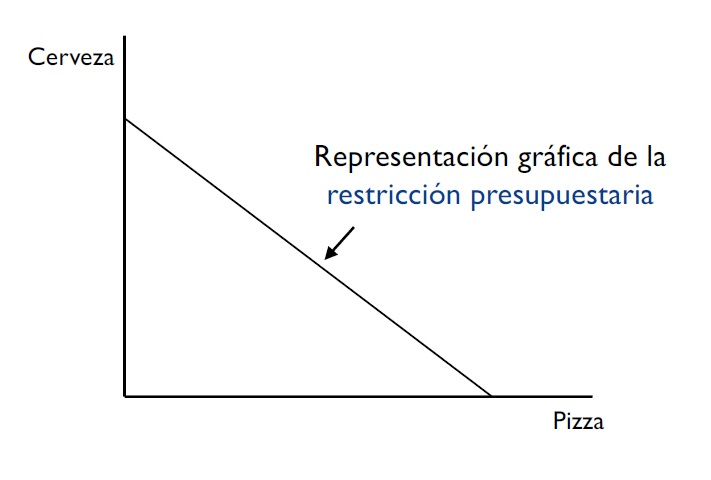
\includegraphics[scale=0.6]{../Figures/Tema_02.4_rp2.jpg}
\end{frame}

\begin{frame}
    \frametitle{Mapa de preferencias}
    \centering
    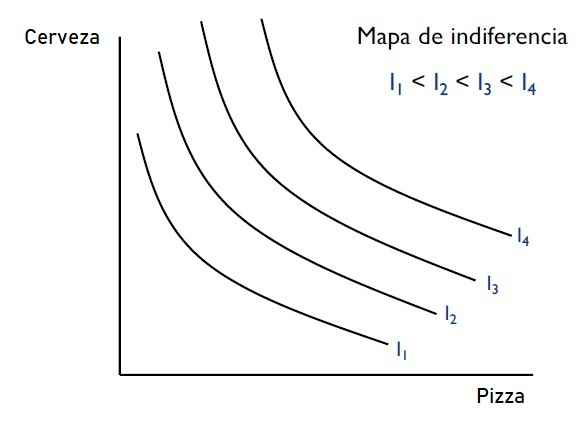
\includegraphics[scale=0.6]{../Figures/Tema_02.16_rp14.jpg}
\end{frame}

\begin{frame}
    La pendiente de la restricción presupuestaria indica la tasa de intercambio a la que el consumidor puede cambiar un bien por otro. 
    \begin{itemize}
        \item Se puede pensar como un costo de oportunidad, como un sacrificio, etc.
        \item Indica también el ratio de precios:
        
        \[Pend = \frac{\Delta Y}{\Delta X} = -\frac{Px}{Py} = TMT\]

        \item La pendiente de la restricción presupuestaria es igual a la tasa marginal de transformación (TMT): La cantidad de un bien que el consumidor \textbf{debe} renunciar para obtener una unidad más del otro bien
        \item Es constante!
    \end{itemize}
\end{frame}

\begin{frame}
    La pendiente de la curva de indiferencia indica la tasa de sustitución a la que el consumidor \textbf{está dispuesto} a cambiar un bien por otro.
    \begin{itemize}
        \item Tiene ciertas propiedades:
        \begin{itemize}
            \item Completitud.
            \item Monotonicidad fuerte.
            \item Transitividad.
            \item Convexidad.
        \end{itemize}
        \item A la pendiente la llamamos también Tasa Marginal de Sustitución.
        
        \[Pend = \frac{\Delta Y}{\Delta X} = - \frac{UMg_x}{UMg_y}\]

        \item La TMS indica cantidad de unidades de un bien que el individuo \textbf{está dispuesto} a sacrificar a cambio de una unidad adicional del otro bien.
        \item No es constante! ¿Intuitivamente, por qué?
    \end{itemize}
\end{frame}

\begin{frame}{Equilibrio}
    \centering
    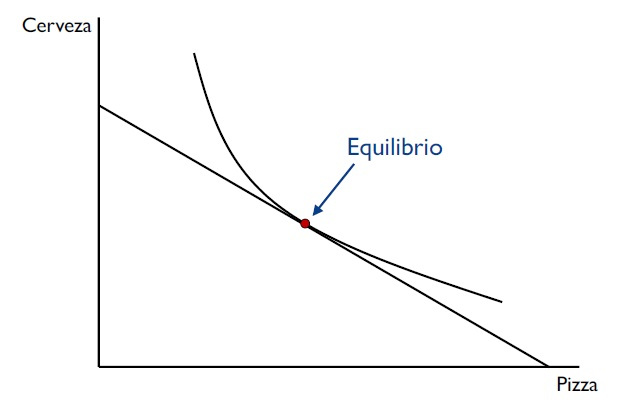
\includegraphics[scale=0.65]{../Figures/Tema_02.19_rp17.jpg}
\end{frame}

\begin{frame}{¿Como decide el consumidor?}
    
    \[TMS = - \frac{UMg_x}{UMg_y}\]
    
    \[TMT = - \frac{P_x}{P_y}\]

    \begin{itemize}
        \item Si $TMS > TMT$, el consumidor está dispuesto a sacrificar más bien Y por una unidad adicional de bien X que lo que el mercado le pide por esa unidad adicional de bien X (estoy del lado derecho del equilibrio!).
        \item Si $TMS < TMT$, el consumidor está dispuesto a sacrificar menos bien Y por una unidad adicional de bien X que lo que el mercado le pide por esa unidad adicional de bien X (estoy del lado izquierdo del equilibrio!).
        \item La canasta óptima es aquella en la que la TMS es igual a la TMT.
    \end{itemize}
\end{frame}
    
\begin{frame}{¿Cómo construir los costos medios?}
    \centering
    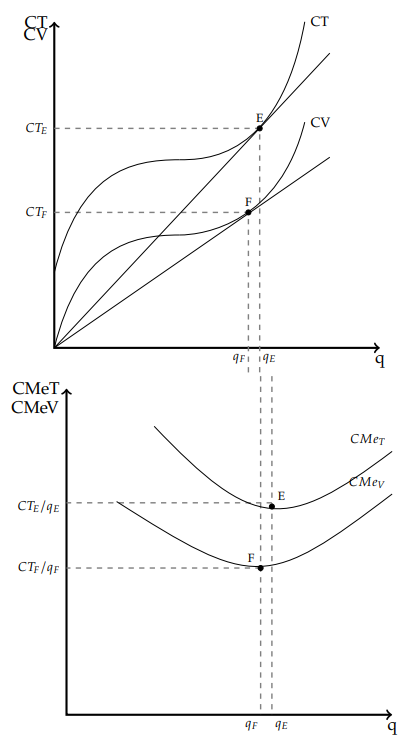
\includegraphics[scale=0.5]{../Figures/C13.6.png}
\end{frame}

\begin{frame}{Graficando costo medio y marginal en el mismo gráfico}
    \centering
    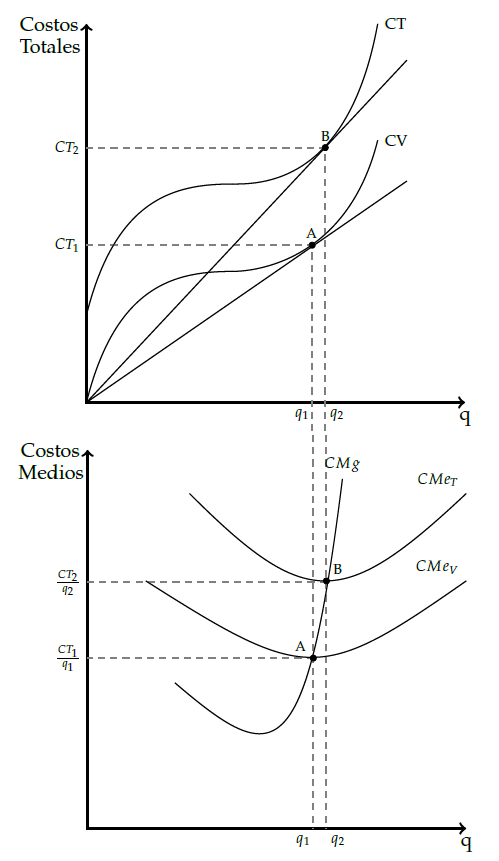
\includegraphics[scale=0.9]{../Figures/Costoscp.png}
    \end{frame}
    
    \begin{frame}
    \frametitle{Las propiedades de las curvas}
    \begin{itemize}
        \item El costo marginal eventualmente aumenta debido a los rendimientos marginales decrecientes.
        \item La curva de costo total promedio suele tener forma de U. Bajan los costos fijos medios y aumentan los costos variables medios.
        \item La curva de costo marginal corta la curva de costo total promedio en su nivel mínimo.
        \item Si el costo marginal es menor al costo medio, el costo medio disminuye al aumentarla producción.
    \end{itemize}
\end{frame}

\begin{frame}{La curva de oferta de la empresa}
    \centering
    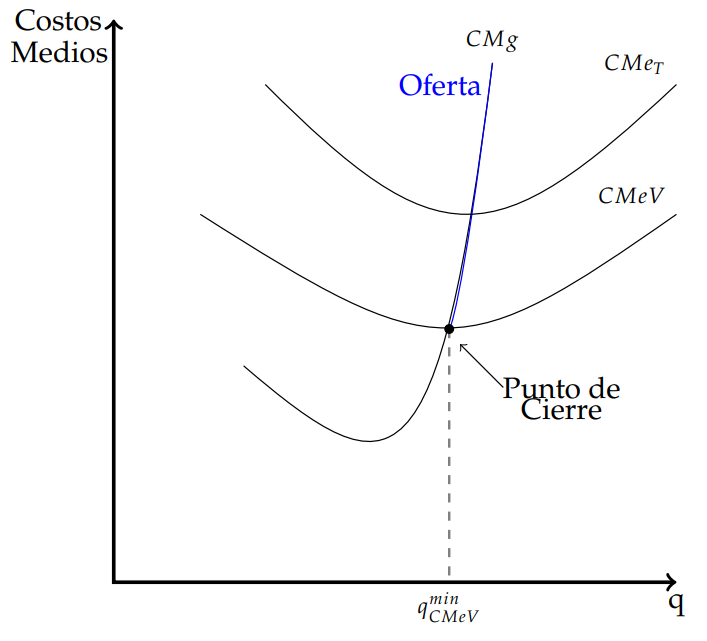
\includegraphics[scale=0.5]{../Figures/C13.11.png}
\end{frame}

\begin{frame}
    \frametitle{Costos en el largo plazo}
    \centering
    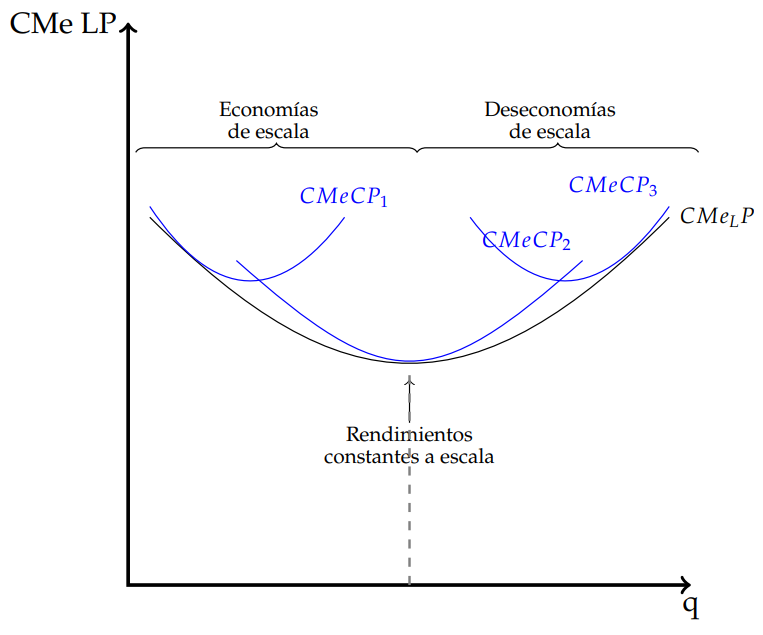
\includegraphics[scale=0.6]{../Figures/C13.10.png}
\end{frame}

\begin{frame}
    \frametitle{Motivación: El precio del petroleo}
    \centering
    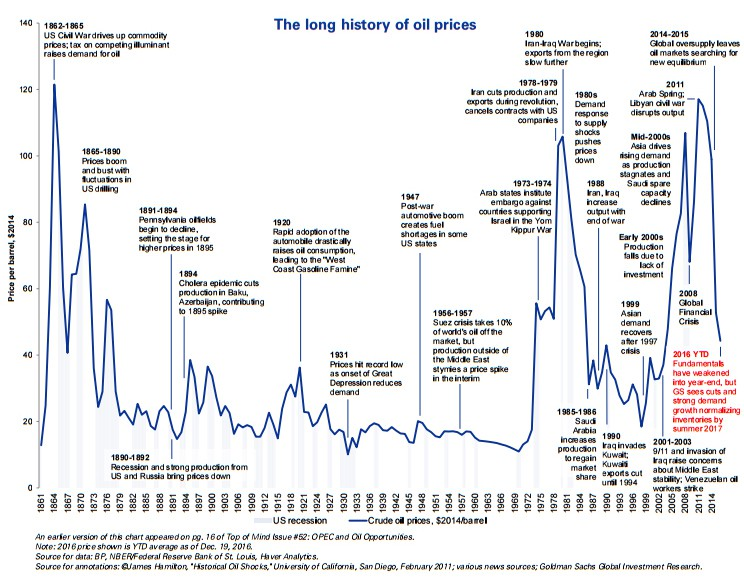
\includegraphics[scale=0.35]{../Figures/Tema_04.01_new.jpg}
\end{frame} 

\begin{frame}{La eficiencia de mercado en términos gráficos}
    \begin{itemize}
      \item A la suma del excedente del consumidor y del productor se la denomina excedente total.
      \item La eficiencia de mercado se refiere a la maximización del excedente total.
      \item Cuando la asignación no es la de equilibrio de mercado, existen ganancias o beneficios no explotados.
    \end{itemize}
    \centering
    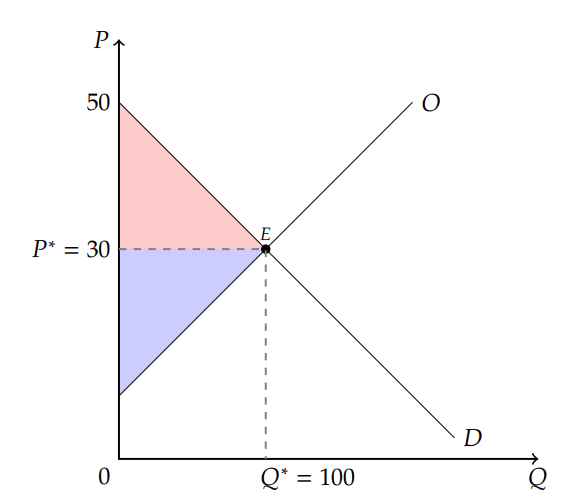
\includegraphics[scale=0.5]{../Figures/C17.9.png}
\end{frame}

\begin{frame}
    \frametitle{Elasticidad precio de la demanda}
    \begin{itemize}
        \item El concepto matemático que los economistas usamos para ver qué tan sensible es la cantidad que se demanda ante un cambio en el precio de un bien se denomina elasticidad precio de la demanda.
        \begin{equation*}
            \epsilon = \left|\frac{- \Delta \% Q}{\Delta \% P}\right| = \left|\frac{\frac{- \Delta Q}{Q}}{\frac{\Delta P}{P}}\right| = \left|-\frac{\Delta Q}{\Delta P} \frac{P}{Q}\right|
        \end{equation*}
        \item Debido a que la cantidad demandada de un bien está negativamente relacionada con el precio del bien, el cambio porcentual en la cantidad siempre tendrá un signo opuesto al del cambio porcentual en el precio.
        \item ¿Como interpretarlo? Como el cambio \% que se produce en la cantidad demandada ante un cambio de 1\% en el precio.
    \end{itemize}
\end{frame}

\begin{frame}
    \frametitle{¿Qué pasa en la empresa?}
    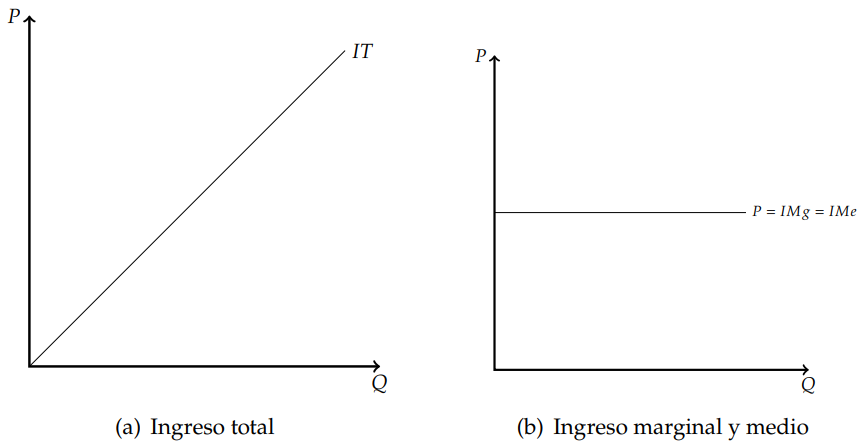
\includegraphics[scale=0.6]{../Figures/C21.4.png}
\end{frame}

\begin{frame}{¿Y en el largo plazo...}
    \begin{center}
    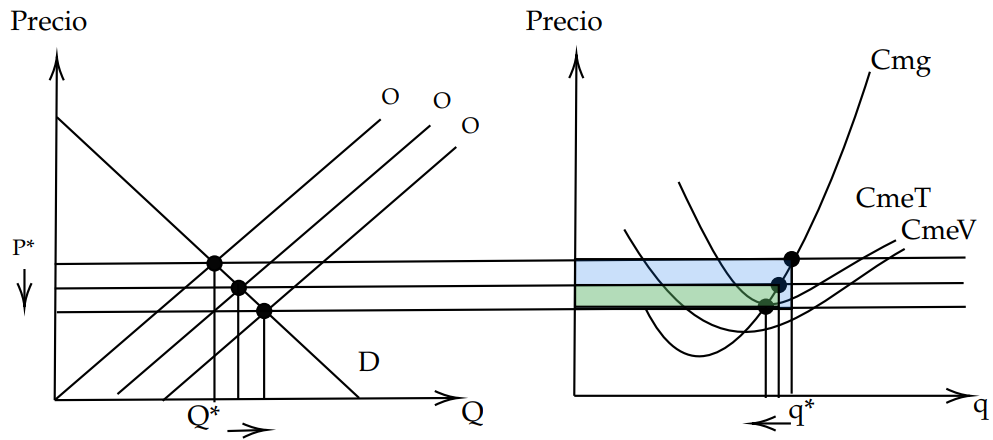
\includegraphics[scale=0.55]{../Figures/C21.6.png}
    \end{center}
\end{frame}

\begin{frame}
    \frametitle{Recordemos lo que sucede en equilibrio... beneficios para todos!}
    \begin{center}
    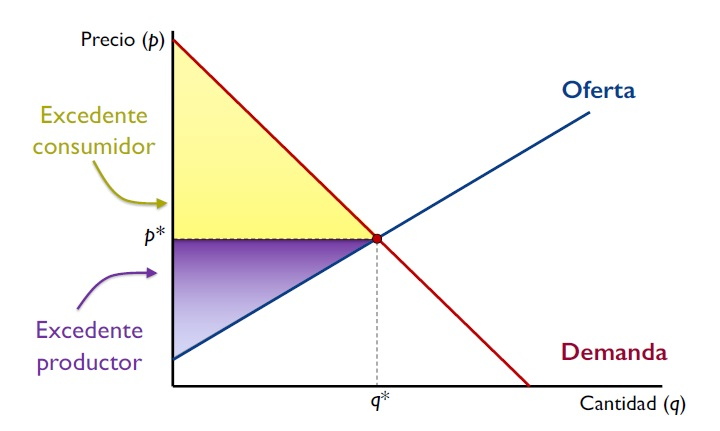
\includegraphics[scale=0.55]{../Figures/Tema_07.23_equilibrioyexcedente.jpg}
    \end{center}
    \end{frame}
    
    \begin{frame}
    \frametitle{¿Por qué es eficiente?}
    \begin{itemize}
        \item Los participantes son tomadores de precios
        \begin{itemize}
            \item No hay poder de mercado.
            \item La competencia impide a los vendedores aumentar el precio, y a los compradores bajarlo.
        \end{itemize}
        \item No hay barreras de entrada
        \item Los contratos son completos
            \begin{itemize}
            \item Los detalles del intercambio pueden ser definidos en forma clara, y estos contratos se pueden hacer cumplir.
            \end{itemize}
        \item No hay externalidades
            \begin{itemize}
            \item La transacción sólo afecta a los compradores y vendedores
            \end{itemize}
    \end{itemize}
\end{frame}

\begin{frame}{Equilibrio del monopolista}
    \centering
    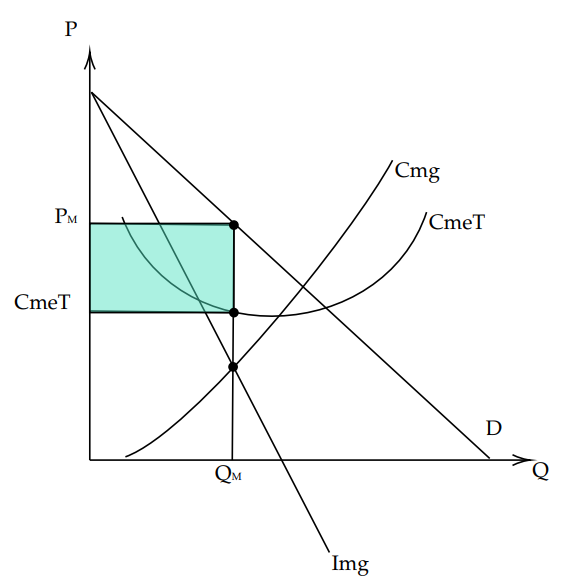
\includegraphics[scale=0.6]{../Figures/C22.5.png}
\end{frame}

\begin{frame}
    \frametitle{Pérdida de eficiencia}
    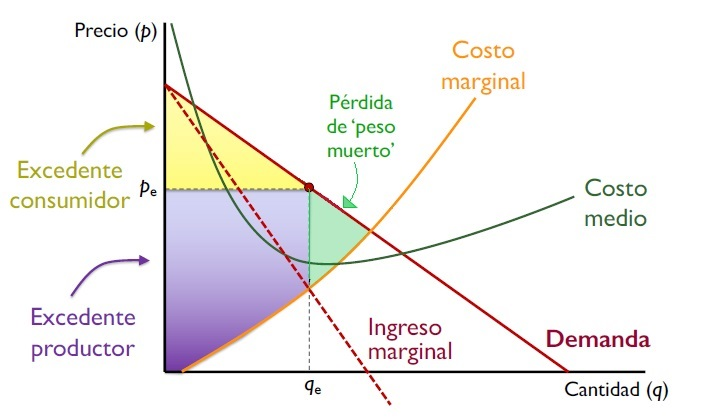
\includegraphics[scale=0.6]{../Figures/Tema_06.42_excedente5.jpg}
\end{frame}

\end{document}